
\documentclass[article,type=bsc,colorback,accentcolor=tud9c]{tudthesis}
%\usepackage{ngerman}
\usepackage{hyperref}
\usepackage{biblatex}
\usepackage{tikz}
\usepackage{listings}
\usepackage{subcaption}
\usepackage{multirow}
\usepackage{amsmath}


\lstdefinelanguage{JavaScript}{
  morekeywords=[1]{break, continue, delete, else, for, function, if, in,
    new, return, this, typeof, var, void, while, with, await, async, case,
    catch, class, const, default, do, enum, export, extends, finally, from,
    implements, import, instanceof, let, static, super, switch, throw, try},
  % Literals, primitive types, and reference types.
  morekeywords=[2]{false, null, true, boolean, number, undefined,
    Array, Boolean, Date, Math, Number, String, Object},
  % Built-ins.
  morekeywords=[3]{eval, parseInt, parseFloat, escape, unescape},
  sensitive,
  morecomment=[s]{/*}{*/},
  morecomment=[l]//,
  morecomment=[s]{/**}{*/}, % JavaDoc style comments
  morestring=[b]',
  morestring=[b]",
  morestring=[b]`
}[keywords, comments, strings]

\lstset{
  language=JavaScript,
  basicstyle=\ttfamily
}


\addbibresource{thesis.bib}

\newcommand{\getmydate}{%
  \ifcase\month%
    \or Januar\or Februar\or M\"arz%
    \or April\or Mai\or Juni\or Juli%
    \or August\or September\or Oktober%
    \or November\or Dezember%
  \fi\ \number\year%
}

\begin{document}
  \thesistitle{Analysis of Methods for Background Execution in Modern Web Applications}%
    {Analyse von Verfahren für Hintergrundausführung in modernen Webanwendungen}
  \author{Yannick Reifschneider}
  \referee{Nikolay Matyunin}{Prof. Dr. Stefan Katzenbeisser}
  \department{Fachbereich Informatik}
  \group{Security Engineering}
  \dateofexam{\today}{\today}
  \tuprints{12345}{1234}
  \makethesistitle
  \affidavit{Yannick Reifschneider}

  \tableofcontents

  \newpage
  \section{Abstract}

  In this thesis we analyse modern browsers regarding their behaviour of JavaScript code exection in background tabs. We show that the energy conserving methods of desktop browsers can easily be circumvented to do arbitrary calculations for unlimited time while the web site is not user visible. With these findings we trace popular websites to see if they use similar methods to execute uninterrupted in the background.

  \newpage
  \section{Introduction}

  Web technology received rapid advances in the last years. Many websites not only deliver static information in form of text and images, but are complete highly dynamic applications which compete with traditional software products. For many of the standard business applications like an E-mail client, a word processor or even a bitmap graphic manipulation software there are alterantives\footnote{\url{https://www.google.com/gmail/about/}}\footnote{\url{https://products.office.com/en-us/free-office-online-for-the-web}}\footnote{\url{https://www.photopea.com/}}, which are developed using web technologies and used via a modern web browser. The web browser has grown from a renderer of static information to the operating system of web applications. Some reasons for the rise of these web applications are, that browsers are getting more capable every year and the JavaScript performance is increasing drastically so that these applications are possible in the first place. Developing a web application instead of traditional software has also many benefits for the developer of said software. Web apps don't need installation, just a modern web browser, which comes preinstalled with any common operating system and mobile device. Visiting a web site to try out a piece of software is a much smaller hurdle to overcome then downloading, installing and running a piece of software. These reasons make the web a popular platform for developing new applications.

  At the same time, the revenue model for many websites is advertising. Websites include third party JavaScript from ad networks, which display ads and track impressions. The included code can be controlled by the advertiser. For a malicous entity, it is therefore possible to include JavaScript on reputable websites just by paying for the ad impression. This method of distribution for malicous script is known as malvertising\cite{wiki:malvertising}.

  The web browser is a fundamental application on most personal computing devices and is trusted by it's users. Because many modern applications are implemented as web apps, web browser usage is ubiquitous in the usage of computing devices. As such, many users leave the web browser open during the whole time they use their device, often times with many website tabs open. The browser vendors are encouraged to conserve as much energy as possible to enable users on battery powered devices, such as mobile phones or notebooks which are not tethered to a power outlet, a longer usage time. On the other side, the browser should not break web applications which require regular CPU time to function correctly. Web apps, which need regular CPU time are sites, which notify the user about new content such as a news site or a social network, a web application which plays audio or video, or a web video conference application. All modern browsers limit the amount of CPU time a tab in the background can use and how often web sites can schedule new work. For maximum energy efficiency, all tabs in the background should eventually be halted completely and only woken up, when the page is moved to the foreground again. This is also the goal of browser vendors\cite{chrome-background-tabs-roadmap}, but the execution of this goal is easy without breaking existing web applications or providing a workaround for some applications.

  In this thesis we find out, if the throttling mechanisms employed by browser vendors can be circumvented, so that web sites which are not visible to the browser can gain code execution for arbitrary time. We compare the different throttling mechanisms between desktop and mobile browsers and we trace popular websites to see if the found cirumvention methods are actively used in the wild.
  
  \subsection{Motivation}

  To render a website, the browser has to execute all JavaScript code which was included in the web site. With browser default settings this happens without the users explicit consent. This means the web site authors can use the browser of it's visitors to execute arbitrary scripts. This very fundamental behaviour of the web is therefor also attracting malicous entities. There are numerous activities, which malicous entities could perform with access to a web site with high amount of daily visits.

  \begin{itemize}
  \item The attacker could inject a browser crypto-currency miner to convert electricity of the website visitors into crypto currency. The existance of crypto currencies such as Monero, which uses proof of work algorithm, which is inefficient to calculate on custom hardware, makes the browser a viable target for such mining. Existing implementations of Monero miners implemented in web assemlby are available for this attack.
  \item The browser could be used as a compute node in a botnet, which can be used for DDoS attacks or for cracking hashed passwords. Grossman et al.\cite{grossmann2013million} show that these attacks can be used with standard web technologies and not exploiting any weaknesses.
  \item The computer of the visitor itself could be compromised by using exploits of the browser or the underlying system itself. Attacks which exploit hardware weaknesses such as Spectre\cite{Kocher2018spectre}, which could allow an attacker to read memory space of other browser tabs, could expose sensitive informations such as passwords or banking information of the uses. Rowhammer\cite{rowhammer} attacks could even persistently infect the users system. These exploits usually need quite some time to be successful and could benefit from constant background execution in a background browser tab.
  \end{itemize}

  

  \subsection{Related works}

  \begin{itemize}

  \item Papadopoulos et al.\autocite{papadopoulos2018truth} analyses the if Cryptocurrency miners are a viable alternative to traditional ad serving as a revenue possibility for web sites. They come to the conclusion, that cryptocurrency mining is more profitable when a user stays longer then 5.3 minutes on the website. When permanent execution of a crypto miners are possible in background tabs, then this time could easily be achieved.

  \item Papadopoulus et al.\cite{papadopoulos2018master} show that browsers can be infected with malicous service workers to act as a puppet in a botnet. Their method for persistence requires an implementation of a draft proposel HTML5 API, which is not implemented in mainstream browsers yet. They focus in their research on service workers, which are independent of browser tabs, but poses other limitations. Our research instead focuses on web sites which are not user visible, i.e. in an inactive tab.   

    
  \item Measurements of existing popular websites is done for privacy related as well as security releated research. Engelhardt et al.\cite{englehardt2016online} for example developed the OpenWPM framework for doing privacy measurements on million of websites. This framework is also used for ...

    Security related analysis of existing webpages are done for example: to measure the use of third party script inclusions\cite{nikiforakis2012you}, to assess the security claims provided by third party security seal providers\cite{van2014clubbing} or to study malware distributed via ad networks\cite{zarras2014dark}.


  \item Pan et al. analyse the feasability to use the browser of website visitors for offloading large computing tasks\cite{pan2015gray}. They termed this usage of distributed data processing gray computing, because it can be done without the users explicit consent, for example while the users are watching video streams. Their research focus is the performance of web workers and the cost effectiveness in comparison to cloud computing offerings. Our research complements the findings of Pan, because they could allow grey computing even when the user is consuming other web sites.

    
  \end{itemize}

  
  \newpage
  \section{Background}

  JavaScript is the only programming language supported by all modern web browsers to enhance web sites or web applocications. If you compare JavaScript to other more traditional programming languages like C, C++ or Java you see some major differences between them.

  \begin{itemize}
  \item JavaScript has no functions for I/O like writing to a file or opening a socket. It depends on a runtime environment like a browser to provide I/O functionality.
  \item JavaScript has no concept of parallelism like operating system threads or processes.
  \item JavaScript is an event driven language and has a built in event loop.
  \end{itemize}

  All of these differences stem from the fact, that JavaScript was designed as an addition to HTML for enhancing web applications and the interface to the browser internal workings, such as the DOM. Many of these design decisions are choosen, because JavaScript is run in the browser and therefore can be run on any website you visit. This poses many security implications, because you may not want to give a website you visit the power to execute arbitrary programms on your computer.

  Also explain why webassembly does nothing special in regards to background execution. That is, because it allows seamleas interop between webasm and Javascript functions. Therefore it has to run with the same runtime guarantees as JavaScript. WebASM Threads are based on Webworkers with a shared memory pool.
  WebASM therefore behaves exactly like javascript functions and have to yield to the event loop to not block the browser.

  
  \subsection{The JavaScript execution model}
  
  
  The JavaScript runtime uses an event loop to schedule tasks for execution\autocite{mdn-event-loop}. The browser or other JavaScript code can put tasks on the task queue. During a single run of the event loop, the runtime removes the first item of the task queue and executes it. When the event queue is empty, the run loop waits until an event is placed into the queue.

  When a JavaScript task is running, it is guaranteed to not be interrupted until it is completed. This insures, that a variable cannot change from outside. This is in contrast to many other programming languages like Java or C, where another thread can mutate variables at any time. To guarantee this behaviour, the JavaScript runtime in the web browser has to block and wait until the task finishes, because the JavaScript task has access to the browser internal state and DOM. Once the task is finished, the runtime can perform other work, such as layout calculations, which mutates its internal state. Due to these properties JavaScript tasks should be as small as possible to ensure responsiveness of the browser. If a JavaScript task takes a long time to complete (i.e. it is executing an infinite loop) most browser show a warning to the user that a script is slowing down the website. The user then has the option to kill the task or wait for the task to finish.
  
  
  \subsection{Web workers}

  Web workers are a mechanism to perform long running uninterruptable calculations. Due to the runtime guarantees which were described in the last section, Web workers have a completely seperate execution context. They don't share variables or resources with the invoking context.

  The web worker and main thread context can communicate by passing messages to each other, which are handled by their respective event loops. In contrast to the main thread, which can manipulate the DOM of the browser, the Web worker has limited functionality. This limitation allows the web worker to run uninterrupted for longer times, because it does not does not block browser events.


  
  \newpage
  \section{Analysis of different background execution methods}

  As we have shown in the motivation section of this thesis, there numerous incentives to execute code in the background. Browsers vendors in contrast are motivated to limit the energy impact of JavaScript code in background tabs as much as possible to prolong the battery life of the users device. To assess the behaviour of the browser throttling mechanisms, we developed a framework to compare different methods for achieving background code execution. The framework handles the benchmarking and visualisation of each method. If new HTML5 APIs are released, that allow for a new method of scheduling tasks, this method can be plugged into the framework to compare it against existing methods. The framework also allows easy reproducability of our analysis, to test whether the throttling mechanisms of browsers changed in new versions. In our analysis we evaluate the throttling mechanisms employed by the following desktop browsers:

  \begin{itemize}
  \item Google Chrome 76
  \item Mozilla Firefox 69
  \item Apple Safari 12.1.2
  \end{itemize}

  For mobile browsers we evaluate these browsers:

  \begin{itemize}
  \item Google Chrome for Android 76
  \item Firefox for Android
  \item iOS 12.4.1 Mobile Safari
  \end{itemize}

  On iOS we only analyse Mobile Safari, because Apple does not allow other browser engines in the Apple AppStore. Every other browser app has to use the system-provided webview to be in accordance with § 2.5.6 from Apple Review Guidelines\footnote{\url{https://developer.apple.com/app-store/review/guidelines/\#software-requirements}}.

  On Android, we can differentiate between different browser engines.
  
  
  \subsection{Methodology}

  In the following sections we look at different methods for scheduling JavaScript code, when the tab is in the background. We describe how each browser behaves when this method is used to execute JavaScript code in the background and we use our measureing framework to compare the browser behaviour for each method.

  The measuring framework takes one parameter, to tune the measuring. With this parameter we can define the workload in milliseconds. This time defines, how long a simulated task should perform uninterrupted work. When this work is performed on the JavaScript main thread then the browser is unresponsive for this amount of time, until the simulated workload finished and yields back to the main thread. Google Chrome advises to keep all JavaScript tasks to under 50ms, to be percieved as immediate for the user\cite{chrome-rail-model}. For our analysis, we measure each method with two workload times for each browser, once for the recommended 50 ms workload and once for a long 1000 ms workload. The measurement is started automatically when the website page is moved to the background and stopped when it is visible again. The framework uses the Page Visibility API \cite{mdn-page-visibility} for determining the current page visibility.

  To test the browsers behaviour to background tasks, we developed a browser automation script using Selenium WebDriver \cite{webdriver}. WebDriver lets us automate different browsers using an API. In our automation script, we open our analysis page which embeds our measuring framework and starts the benchmark by opening a new empty browser tab. After a fixed amount of time, we close the empty browser tab to make the analysis page visible again and therefor stopping the measuring. This procedure is repeated for every browser, with every test method and the two defined workload times.

  After the benchmarking for one scenario is complete, the measuring framework produces a CSV file for downloading the recorded invocations in the background. Each row in the CSV file corresponds to one invocation of the simulated work load. The recorded data includes the time since the web page moved to the background, the time since the last invocation and a computed average CPU usage. This computed CPU usage is derived from the last invocation time and the simulated work load duration with the following formula:

  \begin{equation*}
    CPU_{avg} = \frac{t_{work duration}}{\Delta t_{last invocation}}
  \end{equation*}

  With this data we can then plot the computed CPU usage over time and compare different browsers for each scenario.

  
  \subsection{Timer tasks}

  The default method to schedule new tasks for execution is to use the function \texttt{setTimeout()} or \texttt{setInterval()} which are available on window or worker global scope. These methods take at least two arguments. The first is the function which should be scheduled as a task. The second argument is the time in milliseconds to wait before the task should be executed. As this is the most straighforward way to schedule tasks, this method might be the one which gets throttled the most. The WHATWG specification for timers\cite{whatwg-timers} even explicitly defines an optional waiting time which is user-agent defined to allow for optimization of power usage. Also, when \texttt{setTimeout()} calls are nested or \texttt{setInterval()} repeats the 5th time, the minimum waiting time is incresed to be 4ms.

  Google Chrome throttles timers for a page, when it is in the background or not user visible \cite{chrome-background-tabs}. Since Version 11 timers are batched at most once a second. This batching helps in reducing the battery impact of the background page. Since Version 57 Google Chrome also uses a budget based timer throttling. Budget based timer throttling works by introducing a timer budget for every page in the background. When the web site is in the background for longer then 10 seconds, the budget is considered. Every scheduled timer task is only executed when the budget for this page is greater then zero. The runtime of the task is subtracted from the budget. The budget regenerates for 0.01 seconds per second. This budget based throttling has multiple implications for background pages. First, it allows for sudden bursts in computing time, when these burst are very infrequent, because the budget regenereates continously, and can be depleted in a very short amount. Background web pages which want to use continous computation time, are limited to an average of 1\% of CPU usage over time, because the budget regenerates at a rate of 1/100th of a second per second. The real CPU usage usually is a little higher then 1\% on average though and only approaches 1\% the longer the site is in the background, because the budget can be overdrawn with a long lasting task at the end of the measurement.


  Firefox employs similiar throttling mechanisms to the ones from Google Chrome \cite{mdn-page-visibility}, though the details of the Firefox implementation differ slightly. When a page is in the background, Firefox invokes timers at least one second after the last timer finished. This is in contrast to Googles throttling to invocations once per second. The difference is most visible, when the task duration is 1 sec, because with Googles throttling implementation, the next task fires immediatly, whereas Firefox waits an additional second, before the next task is scheduled. Another differences is, that in Firefox, the budget based timer throttling is used after a page is in the background for 30 seconds, instead of 10 seconds for Google Chrome. Also Firefox caps the page budget at a minimum of -150 ms and a maximum of 50 ms. That means, that Firefox does not allow large burst of tasks, because the budget never increases above 50 ms, but longer lasting tasks, do not overdraw the budget more then -150 ms. This behaviour favors tasks, which are longer then 150ms. For example a repeated task with a duration of 1000 ms only needs to wait for 15 seconds, before it is executed again in Firefox, whereas the same task would have to wait for 100 seconds in Google Chrome, before the budget is posivite again. Firefox also employs additional throttling to tracking scripts \cite{mdn-tracker-throttling}, which limit repeated invocations to known tracker scripts to at most once every 10 seconds.

  Safaris throttling behaviour is different then both Google Chrome's and Mozilla Firefox's behaviour. Scheduled tasks in background pages get invoked by Safari in increasing intervals. This ensures, that the CPU usage for background pages decreases much more rapidly then the CPU usage of the same page in Chrome or Firefox. Safari also coalesces timer calls, to prevent periodic wake ups of the CPU for the invocation of timers. Instead multiple timers are invoked one after the other to then let the CPU move to a energy saving state.

  \textbf{TODO: add iOS and Android}
  
  \begin{figure}
    \begin{subfigure}[t]{0.45\textwidth}
      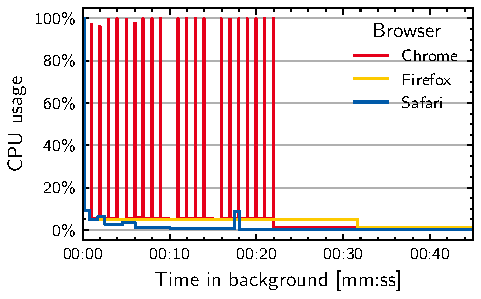
\includegraphics[width=\textwidth]{images/timer-50.pdf}
      \caption{50 ms task duration}
    \end{subfigure}
    \hfill
    \begin{subfigure}[t]{0.45\textwidth}
      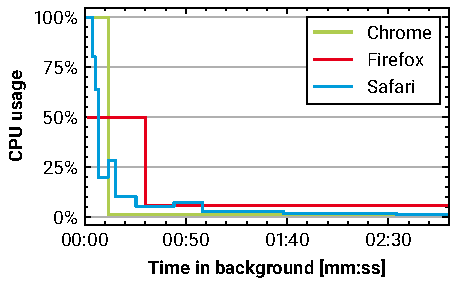
\includegraphics[width=\textwidth]{images/timer-1000.pdf}
      \caption{1000 ms task duration}
    \end{subfigure}

    \caption{CPU usage over time for continuously scheduled timer tasks}
    \label{fig:timer}
  \end{figure}

  \subsection{Timer tasks with WebSocket / AudioContext}

  Browser vendors try to strike a balance between throttling background pages as much as possible to conserve energy and keep the system more responsive and not breaking existing web applications. As backwards compatibility is an important factor, some browsers reduce their throttling, when they detect, that a web application might need more background processing time. The detection, if a web site needs more processing time is difficult though. Due to the dynamic nature of JavaScript, static analysis of web scripts is very difficult. Therefore browsers use a simple heuristic, to determine if their default throttling should be reduced.

  Chrome disables the budget-based throttling, when a web site has either an open WebSocket connection open or plays audible music. Playing silent music does not count as audible music playback though \cite{chrome-background-tabs}. This behaviour could be misused to get more processing time for JavaScript tasks. Playing a audbile sound file or opening a WebSocket connection work equalliy in preventing the budget-based throttling, but they differ hugely in how visible they are to the user of the web page. While playing audio is obviously audible and marks your tab with a speaker icon in the tab bar\footnote{This is a convenience feature for users to quickly find out, which tab is producing the sounds. This is especially useful, if you have many tabs open at the same time.}, opening a websocket connection is invisible to the user and requires no user confirmation. Additionally Chrome prevents automatic playback of audio unless the user has interacted with the site before.

  Firefox also disables the budget-based throttling when a open WebSocket connection is active. \textbf{TODO: Check for Audio Context.}

  Safaris behaviours does not change, when a WebSocket connection is active.

  \begin{figure}
    \begin{subfigure}[t]{0.45\textwidth}
      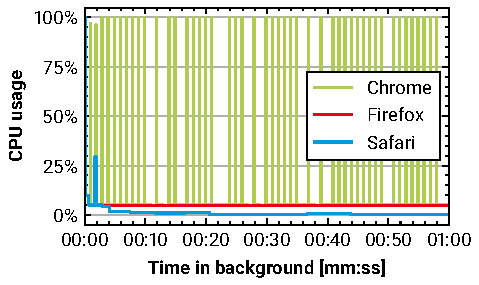
\includegraphics[width=\textwidth]{images/websocket-50.pdf}
      \caption{50 ms task duration}
    \end{subfigure}
    \hfill
    \begin{subfigure}[t]{0.45\textwidth}
      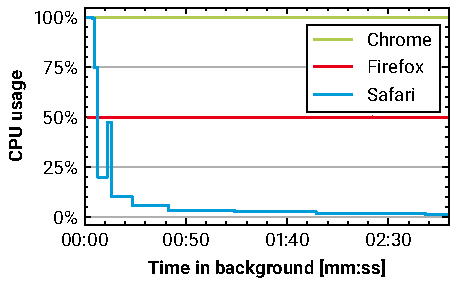
\includegraphics[width=\textwidth]{images/websocket-1000.pdf}
      \caption{1000 ms task duration}
    \end{subfigure}

    \caption{CPU usage over time for continuously scheduled timer tasks during an open WebSocket connection}
    \label{fig:websocket}
  \end{figure}


  \subsection{\texttt{postMessage()} tasks}

  Besides \texttt{setTimeout()} or \texttt{setInterval()} there exists another API for putting tasks in the JavaScript task queue. The function \texttt{postMessage()} available on the window and worker scope is available to allow for communication between windows of different origins or between main thread and worker thread. As each window or worker has its own JavaScript execution context, the communication between these context must happen explicitly via \texttt{postMessage()} calls. The receiving context has to register for the \texttt{message} event on the window or worker object. A call to \texttt{postMessage()} with the receiver set to a window or worker who registered for the event, adds a new task to the task queue for this window. The scheduling of tasks, which are created with the before mentioned method, are not subject to the throttling as explained in the timer tasks section. This is also true for when a \texttt{postmessage()} call is sent and received from the same context. Tasks created with this method are also not subject to the minimum delay of 4 ms as timer tasks are \cite{zero-delay-timeouts}.

  All desktop browsers do not throttle the scheduling of task created via \texttt{postMessage()}. This allows a web site to fully utilize the CPU even when it is on the background. Chrome and Firefox allow to use this method to run indefinitely, whereas Safari detects that a web page is using significant energy and reloads the page after around 8 minutes in the background.

  With this API not being throttled when a web site is in the background, a malicous entity could use this to their advantage. This shows, that the throttling mechanisms put in place for timer tasks are only considered for saving energy for well-behaving websites and not for protecting the users web sites which actively try to circumvent the throttling.
  

  
  \subsection{Web workers}
  
  Using the worker-timers\footnote{\url{https://github.com/chrisguttandin/worker-timers}} library to run a scheduler on a web worker, which calls a callback on the main loop. This circumenvents the setInterval throttling, when a browser tab is in the background.
  
  \subsection{Service workers}

  Service workers have advantages. They run independent of the browser tab. They stay can stay aliver after the browser tab, which installed the service worker is closed.

  \begin{itemize}   
  \item Multiple methods for background execution:

  \item Simple set interval after activation

  \item In response to network request (corresponding website has to be open to trigger a network call)

  \item Website push notifications (has to be allowed by user)

  \item Web Background Synchronization API\footnote{\url{https://wicg.github.io/BackgroundSync/spec/}}
  \end{itemize}

  

  Safari reloads background tabs which use too much energy after around 8 minutes with the message ``This webpage was reloaded because it was using significant energy.''.

  \subsection{Summary}

  \begin{table}
    \centering
    \begin{tabular}{ c | p{4,5cm} | p{4,5cm} | p{4,5cm} }
      \multirow{2}{*}{Method} & \multicolumn{3}{c}{Browser} \\
      \cline{2-4}
                              & \multicolumn{1}{|c|}{Google Chrome} & \multicolumn{1}{|c|}{Mozilla Firefox} & \multicolumn{1}{|c|}{Apple Safari} \\
      \hline
      Timers & Coalesced invocations at most once per second.
               Budget-based throttling after 10 seconds in background.
                              & Next invocation at least one second after last invocation.
                                Capped budget-based throttling after 30 seconds in background.
                              & Coalesced invocations. Time between invocations increases. \\
      \hline
      Timers+WS
                              & Coalesced invocations at most once per second. No budget-based throttling.
                              & Next invocation at least one second after last invocation. No budget-based throttling.
                              & Coalesced invocations. Time between invocations increases. \\
      \hline
      \texttt{postMessage}    & No throttling
                              & No throttling
                              & No throttling, but page gets reloaded when it is using significant energy \\
      \hline
      Web Worker              & No throttling
                              & No throttling
                              & No throttling, but page gets reloaded when it is using significant energy
    \end{tabular}
    \caption{Summary of desktop browser throttling behaviour}
    \label{tab:browser-throttling}
  \end{table}
 
  


  \newpage
  \section{Tracing of background execution on popular websites}

  In the first part of this thesis, we identified different methods to circumvent the default browser throttling mechanisms. With these findings in mind we can now trace popular websites\footnote{We used the first one thousand web sites of the Alexa Top 1m Website list} to analyse if these circumenvtion methods are used in the wild. Using the Alexa Top 1 million website list, we measure the average CPU usage of the websites. When we aggregate these tracing result, we can determine, if the browser throttling mechanisms are suiteable to limit CPU usage or if websites use these methods to actively or inadvertently bypass the background throttling mechanisms.
  
  \subsection{Automated measuring of background execution}

  To automate the tracing of popular websites we used the Puppeteer\cite{pptr} library to control and automate Google Chrome. We choose Puppeteer because it allows us to access the Chrome internals like Web Profiler and also inject custom scripts into the loaded page to detect if circumvention methods which are described in part one of this thesis are being used. Puppeteer only allows to control Google Chrome, but with Google Chrome having the greatest market share among common Web browsers this is not a limiting factor.

  The general idea for the tracing is, that we open a new Chrome instance and start the web profiling. Then we open the website to trace and wait for the initial load to complete. After that we move this website to the background by opening a new tab, so that the browser throttling mechanisms are activated. We profile the page for a 15 minutes time period. After the 15 minutes are completed, we close the browser instance and save the website trace for analysis.

  The website trace allows us to understand if the website is running JavaScript code while it is in the background and which methods it used to initiate the execution. On a invidual site level the website trace profile allows us to see, which JavaScript functions were run and how long they took to complete.

  The website trace profile allows us to dig deep into what a single website is executing while it is in the background. But to get a better picture of how popular websites in general behave in the background we have find a way to aggregate the analysis of the traces.

  We propose to use the average CPU usage during the profiling to use as a score for a single website. The average CPU score can be calculated from the trace file by calculating summed duration, in which the website executed JavaScript code in the main thread and in spawned worker threads and dividing the sum by the time the trace was running. Wall clock time is a suitable replacement for CPU time in a scenario where the machine on which the measurements are taken is not under any other load from other processes. A website which uses no JavaScript at all should therefore receive a score of 0, whereas a website which does run uninterupted calculations on the main thread should receive a score of 1. If a website uses multiple worker threads and the machine on which the measurements are taken has more then one physical CPU core, then the website could receive a score which is greater then 1, because all workers could be active at the same time.

  The background throttling mechanism put in place by Google Chrome does limit the timers of websites based on a CPU time budget. This budget is currently set so that websites on average only use 1\% of CPU usage. That would equal a score of 0.01 in our proposed metric. This limit gives a good estimation, if websites try to overcome the background throttling mechanism of Chrome. Websites which score greater then 0.01 presumably use one or more methods to prevent the throttling.

  


  
  \newpage
  \section{Evaluation of tracing results}
  
  \newpage
  \section{Conclusion}

  
  \newpage
  \printbibliography[heading=bibnumbered]

   

\end{document}
